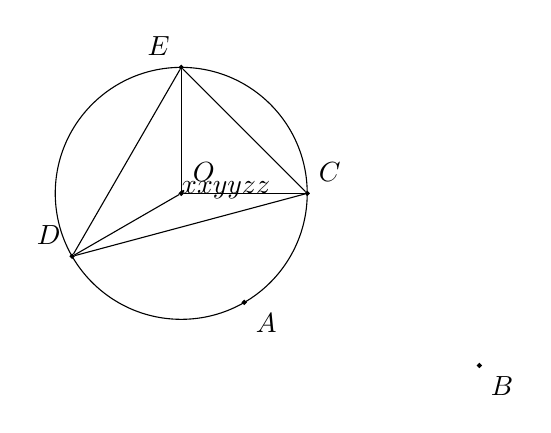
\begin{tikzpicture}
[scale=0.4,>=stealth,point/.style={draw,circle,fill = black,inner sep=0.5pt},]
%\tikzset{shift={(-3,0)}}

%innput parameters
\def\r{4}

%Labeling points
% r sin(pi/3) = 3.4641
\node (O) at (0,0)[point,label=above right:$O$] {};
\node (C) at (\r, 0 )[point,label=above right:$C$] {};
\node (A) at ({\r/2},-3.4641)[point,label=below right:$A$] {};
\node (D) at (-3.4641 , -{\r/2})[point,label=above left:$D$] {};
\node (E) at (0 , \r)[point,label=above left:$E$] {};
\node (B) at (9.4641 , -5.4641)[point,label=below right:$B$] {};


%A



%Drawing parallelogram ABCD
%\draw (O) -- (A);
\draw (O) -- (C);
\draw (O) -- (E);

\draw (E) -- (D);
\draw (D) -- (C);
\draw (E) -- (C);
\draw (O) -- (D);
%\draw (D) -- (B);
%\draw (E) -- (B);


\draw (O) circle (\r);
%marking angles
%\tkzMarkAngle[fill=orange!0.5,size=0.003cm,mark=](C,D,O)
%\tkzMarkAngle[fill=green!60,size=0.003cm,mark=](O,C,D)
%\tkzMarkAngle[fill=green!0.5,mark=](O,D,E)
%\tkzMarkAngle[fill=green!0.5,mark=](D,E,O)
%\tkzMarkAngle[fill=green!0.5,mark=](O,E,C)
%\tkzMarkAngle[fill=green!0.5,mark=](E,C,O)
\tkzLabelAngle[pos=1.90](C,D,O){$x$}
\tkzLabelAngle[pos=1.90](O,C,D){$x$}
\tkzLabelAngle[pos=1.30](O,D,E){$y$}
\tkzLabelAngle[pos=1.30](D,E,O){$y$}
\tkzLabelAngle[pos=1.00](O,E,C){$z$}
\tkzLabelAngle[pos=1.00](E,C,O){$z$}

%
\end{tikzpicture}
